
\documentclass{jsarticle}
\usepackage[dvips]{graphicx}
\usepackage{amsmath}
\usepackage{longtable}
\usepackage{amsfonts}
\usepackage{amssymb}
\usepackage{comment}
\usepackage{url}
\input{symbol}
% �C�m�_���pA4�T�C�Y�t�@�C���B
%
% HORIZONTAL FEATURES -------------------
\oddsidemargin -1mm
\evensidemargin -1mm
\textwidth 162mm
%
% VERTICAL FEATURES -------------------
\topmargin -18mm
\headheight 6mm
\headsep 8mm
\textheight 245mm
%\footheight  5mm    %% Never used in LaTeX2e
\footskip 15mm

%Fig,Table�p��o��
\makeatletter
\def\fnum@figure{Fig.~\thefigure}
\makeatletter
\def\fnum@table{Table~\thetable}

%�y�[�W���C�A�E�g
\setlength{\voffset}{0.0in}
\setlength{\textheight}{680pt}
\setlength{\hoffset}{-10.0pt}
\setlength{\marginparsep}{0pt}

\renewcommand{\tablename}{Table~}
\renewcommand{\figurename}{Fig.~}
\bibliographystyle{plain}


\title{ODE \cite{WebSmith} でやっている剛体動力学演算を考えてみる}
\author{菱沼 徹}
\date{\today}
\begin{document}
\maketitle

まとめ
\begin{itemize}
\item 力ベース(2階差分方程式)ではなく,撃力ベース(1階差分方程式)
\item 3種類の拘束(等式幾何拘束・不等式幾何拘束・不等式速度拘束)が存在する.
\item 数値誤差に対処する方法として,バウムガルデ法とペナルティ法が存在する.ODEの中では,ERPとCFMがこれに対応する.
\end{itemize}

\section{数学の知識}
\paragraph{ブロック行列}
ブロック行列の逆行列は,$\vD$が逆可能である時,次のように与えられる.
\begin{align*}
   \left(
    \begin{array}{cc}
       \vA   & \vB\\
       \vC   & \vD
    \end{array}
   \right)^{-1}
&=
   \left(
    \begin{array}{cc}
       \vM   & -\vM\vB\vD^{-1}\\
       \vD^{-1}\vC\vM   & \vD^{-1}+\vD^{-1}\vC\vM\vB\vD^{-1}
    \end{array}
   \right)
 ,\hspace{10mm} (\mbox{ ただし }\vM=(\vA-\vB\vD^{-1}\vC)^{-1})
\end{align*}
また,$\vD=\vO$である時は,次のように与えられる.
\begin{align*}
   \left(
    \begin{array}{cc}
       \vA   & \vB\\
       \vC   & \vO
    \end{array}
   \right)^{-1}
&=
   \left(
    \begin{array}{cc}
       \vA^{-1}-\vA^{-1}\vB\vN\vC\vA^{-1}   & -\vA^{-1}\vB\vN\\
       \vN\vC\vA^{-1}   & -\vN
    \end{array}
   \right)
 ,\hspace{10mm} (\mbox{ ただし }\vN=(\vC\vA^{-1}\vB)^{-1})
\end{align*}


\paragraph{LCP}
行列$\vA$,ベクトル$\vb$が既知であるとする.
次式を満たす$\va,\vf$を求める問題を,線形相補計画問題(LCP)という.
\begin{align*}
\va &= \vA \vf + \vb\\
\va &\ge\0,
\hspace{10mm}\vf \ge\0,
\hspace{10mm}\va^T\vf=0\notag
\end{align*}
また,相補条件が未知量の一部のみに課されている場合の問題を,混合線形相補性問題(MLCP)という.
\begin{align*}
   \left(
    \begin{array}{c}
       \0\\
       \va_2
    \end{array}
   \right)
&=
   \left(
    \begin{array}{cc}
       \vA_{11}   & \vA_{12}\\
       \vA_{21}   & \vA_{22}
    \end{array}
   \right)
   \left(
    \begin{array}{c}
       \vf_1\\
       \vf_2
    \end{array}
   \right)
+\vb\\
\va_2 &\ge\0,
\hspace{10mm}\vf_2 \ge\0,
\hspace{10mm}\va_2^T\vf_2=0\notag
\end{align*}


\section{ニュートン・オイラー方程式:ホロノミック拘束(\cite{Book2006JSME},Sec.~13.4.3)}
一般化座標を$\vq$を,位置$\vr_i$とオイラーパラメータ$\vepsilon_i$の組とする.
$m$個の等式幾何学的拘束を,$\vc(\vq)=\0$によって表す.
拘束を破らない微小仮想変位$\delta \vq$は,次を満たす.
\begin{align*}
\frac{\partial \vc}{\partial \vq} \delta \vq = \frac{\partial \vc}{\partial \vr} \delta \vr + \frac{\partial \vc}{\partial \vepsilon} \delta \vepsilon = \vC_r\delta \vr + \vC_\epsilon\delta \vepsilon = \0
\end{align*}
仮想回転変位を$\delta\theta$とおくと,
\begin{align*}
\vC_r\delta \vr + \vC_\epsilon \frac{1}{2}\vL^T \delta \vtheta = \vC_r\delta \vr + \vC_\theta \delta \vtheta =\0
\end{align*}
仮想変位と仮想回転は,拘束条件下で仮想仕事をしないので,拘束力$\vf^{(c)}$,拘束トルク$\vtau^{(c)}$は次を満たす.
\begin{align*}
\vf^{(c)T}\delta \vr + \vtau^{(c)T} \delta \vtheta = 0
\end{align*}
ダランベールの原理より,外力$\vf^A$・外トルク$\vtau^A$・未定乗数$\vlambda$(つまり拘束力)とすると,次が成り立つ.
\begin{align}
[\vM'\dot{\vv}-\vf^A+\vC_r^T\vlambda]^T\delta \vr + [\vI\dot{\vomega}+\vomega\times\vI\vomega-\vtau^A+\vC_\theta^T\vlambda]^T\delta \vtheta = 0
\end{align}
また,拘束条件式$\vc=\0$を2回微分すると,次が得られる.
\begin{align}
\0
&=\frac {d^2\vc}{dt^2}\notag\\
&=\frac {d(\vC_r\vv + \vC_\theta\vomega)}{dt}\notag\\
&=\vC_r\dot{\vv} + \vC_\theta\dot{\vomega} + \dot{\vC}_r\vv+\dot{\vC}_\theta\vomega
\end{align}
これら2つの式を合わせると,系の動力学解析をすることができる.
変数は$(\dot{\vv}^T~\dot{\vomega}^T~\vlambda^T)^T$であり,このような方法は"拡大法"として知られる.
\begin{align*}
   \left(
    \begin{array}{ccc}
       \vM'   & \0        & \vC_r^T\\
       \0    & \vI       & \vC_\theta\\
       \vC_r & \vC_\theta & \0
    \end{array}
   \right)
   \left(
    \begin{array}{c}
       \dot{\vv}\\
       \dot{\vomega}\\
       \vlambda
    \end{array}
   \right)
=
   \left(
    \begin{array}{c}
       \vf^A\\
       \vtau^A-\vomega\times\vI\vomega\\
       -(\dot{\vC}_r\vv + \dot{\vC}_\theta\vomega)
    \end{array}
   \right)
\end{align*}
以降,記号の簡単のため,上式を次で表す.
\begin{align}
   \left(
    \begin{array}{cc}
       \vM   & \vJ^T\\
       \vJ   & \0
    \end{array}
   \right)
   \left(
    \begin{array}{c}
       \dot{\vu}\\
       \vlambda
    \end{array}
   \right)
=
   \left(
    \begin{array}{c}
       \vQ^A\\
       -\dot{\vJ}\vu
    \end{array}
   \right)\label{NE_equation}
\end{align}


\section{拘束条件の安定化方法(ホロノミック拘束)}
式(\ref{NE_equation})では,拘束条件$\vc=\0$を2階微分した式$\ddot{\vc}=\0$を,時刻$t=0$で初期条件$\dot{\vc}=\0,~\vc=\0$として解いている.
つまり,拘束条件$\vc=\0$そのものが成り立つようにして解いているわけではない.
もし仮に厳密に解くことができるとすれば,全ての時刻$t$で$\vc=\0$と拘束が満たされる.
しかし,丸め誤差などによる摂動が加わり$\ddot{\vc}=\vepsilon$となっている場合は,時刻$t$における拘束条件式は$\vc=\frac{1}{2}t^2\vepsilon $となってしまい,時刻$t$に関して2次で増加する(\cite{Book2003JSME},Sec.~7.2.3).

積分誤差の累積を0に引き戻し,拘束式の安定化を図る方法として,次が挙げられている(\cite{Book2007JSME}, Sec.~7.4.3).
\begin{itemize}
 \item バウムガルテ法
 \item ペナルティ法
\end{itemize}

\paragraph{バウムガルテ法}
ニュートン・オイラー方程式と合わせる式として,拘束式の2階微分$\ddot{\vc}=\0$ではなく,次式を用いると優れた拘束安定化が得られる.
\begin{align*}
\0
&= \ddot{\vc} + 2\beta \dot{\vc} + \gamma^2\vc \\
&= \vJ\dot{\vu}+\dot{\vJ}\vu + 2\beta\vJ\vu + \gamma^2\vc
\end{align*}
ここで,$\beta>0$と$\gamma\neq 0$は任意に選ばれた定数である.
この一般解は次であり,時間とともに増大することなく安定する.
\begin{align*}
 \vc = \vc_1\exp^{(-\beta+\sqrt{\beta^2-\gamma^2})t}+\vc_2\exp^{(-\beta-\sqrt{\beta^2-\gamma^2})t}
\end{align*}
運動を得るために解くべき式は,次のようになる.
\begin{align}
   \left(
    \begin{array}{cc}
       \vM   & \vJ^T\\
       \vJ   & \0
    \end{array}
   \right)
   \left(
    \begin{array}{c}
       \dot{\vu}\\
       \vlambda
    \end{array}
   \right)
=
   \left(
    \begin{array}{c}
       \vQ^A\\
       -\dot{\vJ}\vu-2\beta\vJ\vu-\gamma^2\vc
    \end{array}
   \right)\label{Baumgarte_method}
\end{align}

\paragraph{ODEとの対応.}
ODEでは, ERP ( Error Reduction Parameter )を用いている.
これは,バウムガルテ法の単純なバージョンと考えることができる(\cite{MThesis2005Garstenauer}, Sec.~5.2.1).
ODEでは,拘束条件の一回微分$\dot{\vc}$を,運動方程式と連立して解いている(撃力ベース法).
拘束を安定して解くために,代わりに次の拘束条件を解いている.
\begin{align*}
 \0=\dot{\vc} + \frac{ERP}{\Delta t}\vc = \vJ\vu + \frac{ERP}{\Delta t}\vc
\end{align*}

\paragraph{ペナルティ法}
拘束式$\vc$は,常に0になるべきベクトル量である.
数値積分の過程で$\0$から離れた場合を人工的なエネルギーが増加したととらえ,これを0に向かわせるような力を拘束力として系に与える.
(拘束にめり込んだ分だけバネダンパで反力を与えるというのは,ペナルティ法のこと)

人工ポテンシャルエネルギー
\begin{align*}
 P_C=\frac{1}{2}\vc^T\valpha\vOmega^2\vc
\end{align*}
人工運動エネルギー
\begin{align*}
 K_C=\frac{1}{2}\dot{\vc}^T\valpha\dot{\vc} = \vu^T\vJ^T\valpha\vJ\vu
\end{align*}
より,ラグランジュ関数$L_c=K_c-P_c$を定義すると,ラグランジュ方程式より
\begin{align*}
 \vQ_C
&= \frac{d}{dt}\biggl(\frac{\partial L_c}{\partial \vu}\biggr) - \frac{\partial L_c}{\partial \vq}\\
&= \frac{d}{dt}(\vJ^T\valpha\vJ\vu) -\frac{\partial}{\partial \vq}(\frac{1}{2}\vu^T\vJ^T\valpha\vJ\vu) + \vJ^T\valpha\vOmega^2\vc\\
&= \vJ^T\valpha\vJ\dot{\vu} + \vJ^T\valpha\dot{\vJ}\vu + \vJ^T\valpha\vOmega^2\vc
\end{align*}
また,レイリー消散力も人工的に与える.
\begin{align*}
 \vQ_R = 2\vJ\valpha\vOmega\vmu\dot{\vc}
\end{align*}
人工的に考えた拘束力$\vQ_C,~\vQ_R$を運動方程式に加えると,次のようになる.
\begin{align}
 \vM\dot{\vu} &= \vQ^A-\vQ_C-\vQ_R\notag\\
 (\vM+\vJ^T\valpha\vJ)\dot{\vu} &= \vQ^A-\vJ^T\valpha(\dot{\vJ}\vu+2\vOmega\mu\vJ\vu+\vOmega^2\vc)\label{penalty_method}
\end{align}
$\valpha,\vOmega,\vmu$は対角行列である.対角成分は任意に決められるが,実用的には次のように選定される場合が多い.
\begin{align*}
 \valpha = \frac{1}{\epsilon}\vI,~~~~~\vOmega=\omega\vI,~~~~~\vmu=\vI~~~~~~~~~(\vI\mbox{は恒等行列})
\end{align*}

\paragraph{ODEとの対応.}
ODEにおいて用いられる拘束力混合( CFM : Constraint Force Mixing ) は,ペナルティ法(\ref{penalty_method}の一種とみることもできる.
ニュートン・オイラー方程式と合わせる式として,拘束の2階微分$\ddot{\vc}=\0$ではなく,次式を用いる事を考える.
\begin{align*}
 \ddot{\vc} + 2\vOmega\vmu \dot{\vc} + \vOmega^2\vc - \valpha^{-1}\vlambda
=\vJ\dot{\vu}+\dot{\vJ}\vu  +2\vOmega\vmu\vJ\vu + \vOmega^2\vc - \valpha^{-1}
=\0
\end{align*}
このとき,運動を得るために解くべき式は,次のようになる.
\begin{align}
   \left(
    \begin{array}{cc}
       \vM   & \vJ^T\\
       \vJ   & -\valpha^{-1}
    \end{array}
   \right)
   \left(
    \begin{array}{c}
       \dot{\vu}\\
       \vlambda
    \end{array}
   \right)
=
   \left(
    \begin{array}{c}
       \vQ^A\\
       -\dot{\vJ}\vu-2\vOmega\vmu\vJ\vu-\vOmega^2\vc
    \end{array}
   \right)\label{cfm_method}
\end{align}
ブロック行列の逆行列の式を用いると,加速度$\dot{\vu}$は,ペナルティ法(\ref{penalty_method})と同じものが得られる.
\begin{align*}
\dot{\vu} &= (\vM+\vJ^T\valpha\vJ)^{-1}\Biggl[\vQ^A-\vJ^T\valpha(\dot{\vJ}\vu+2\vOmega\vmu\vJ\vu+\vOmega^2\vc) \Biggr]
\end{align*}


\section{不等式幾何拘束とMLCP ( \cite{MThesis2005Garstenauer}, Sec.~4.6.2 )}
$k$番目の接触において,接触する2剛体の接触点を$\vx_{ki},~\vx_{kj}$で表し,接触面の法線ベクトルを$\vn_k$で表すとする.
接触の不等式拘束を次式で置く場合を考える.
\begin{align*}
 c_k=(\vx_{ki}-\vx_{kj})^T\vn_k\ge0
\end{align*}
接触点$k$における拘束力を$\lambda_k$で表し,これを集めたベクトルを$\vlambda$とする.
接触面法線方向への接触点の相対加速度を集めたベクトルは,$\ddot{\vc}=\vJ\dot{\vu}+\dot{\vJ}\vu$によって与えられる.
「各接触点$k$において接触する剛体はめり込む方向へは加速しない」という条件は,$\ddot{c}_k\ge0$によって与えられる.
「各接触点$k$において垂直抗力は反発方向にのみはたらく」という条件は,$\lambda_k\ge0$によって与えられる.
「拘束力は互いに離れていない場合にのみはたらく」という条件は,$\ddot{c}_k\lambda_k=0$によって与えられる.
これらをまとめると,次のようになる.
\begin{align*}
 \ddot{\vc}\ge\0,
 \hspace{10mm}\vlambda\ge\0,
 \hspace{10mm}\vlambda^T\ddot{\vc}=0
\end{align*}
もともと考えたい幾何学的拘束を,運動方程式と連立して解くために,加速度レベルの拘束に書き換えている.
Sec.~2のように,上の条件を運動方程式と合わせて解こうとする場合,次のMLCPを考えることになる.
\begin{align}
   \left(
    \begin{array}{c}
       \0\\
       \ddot{\vc}
    \end{array}
   \right)
=
   \left(
    \begin{array}{cc}
       \vM   & \vJ^T\\
       \vJ   & \0
    \end{array}
   \right)
   \left(
    \begin{array}{c}
       \dot{\vu}\\
       \vlambda
    \end{array}
   \right)
-
   \left(
    \begin{array}{c}
       \vQ^A\\
       -\dot{\vJ}\vu
    \end{array}
   \right)\label{NE_equation''}
\end{align}
\begin{align*}
 \ddot{\vc}\ge\0,
 \hspace{10mm}\vlambda\ge\0,
 \hspace{10mm}\vlambda^T\ddot{\vc}=0
\end{align*}


\section{垂直抗力と摩擦のモデル(不等式速度拘束)}
クーロン摩擦のモデルの条件は,次のように表すことができる.
\begin{align*}
 c_{t,x}^2+c_{t,y}^2\le \mu^2c_n^2
\end{align*}
摩擦力の大きさは,最大静止摩擦力$\mu c_n$より小さいということを意味している.
またこのモデルでは,最大静止摩擦力と動摩擦力は等しいとする.
拘束力$c_n,c_{t,x}, c_{t,y}$についての条件は摩擦円錐 ( friction cone ) によって表現できるが,非線形であるためMLCPでは扱えない.
そのため,\cite{CMAME1999Anitescu}, \cite{IJNME1996Stewart} などでは摩擦円錐を角錐で近似しようと考える.

\begin{figure}[tb]
  \begin{center}
    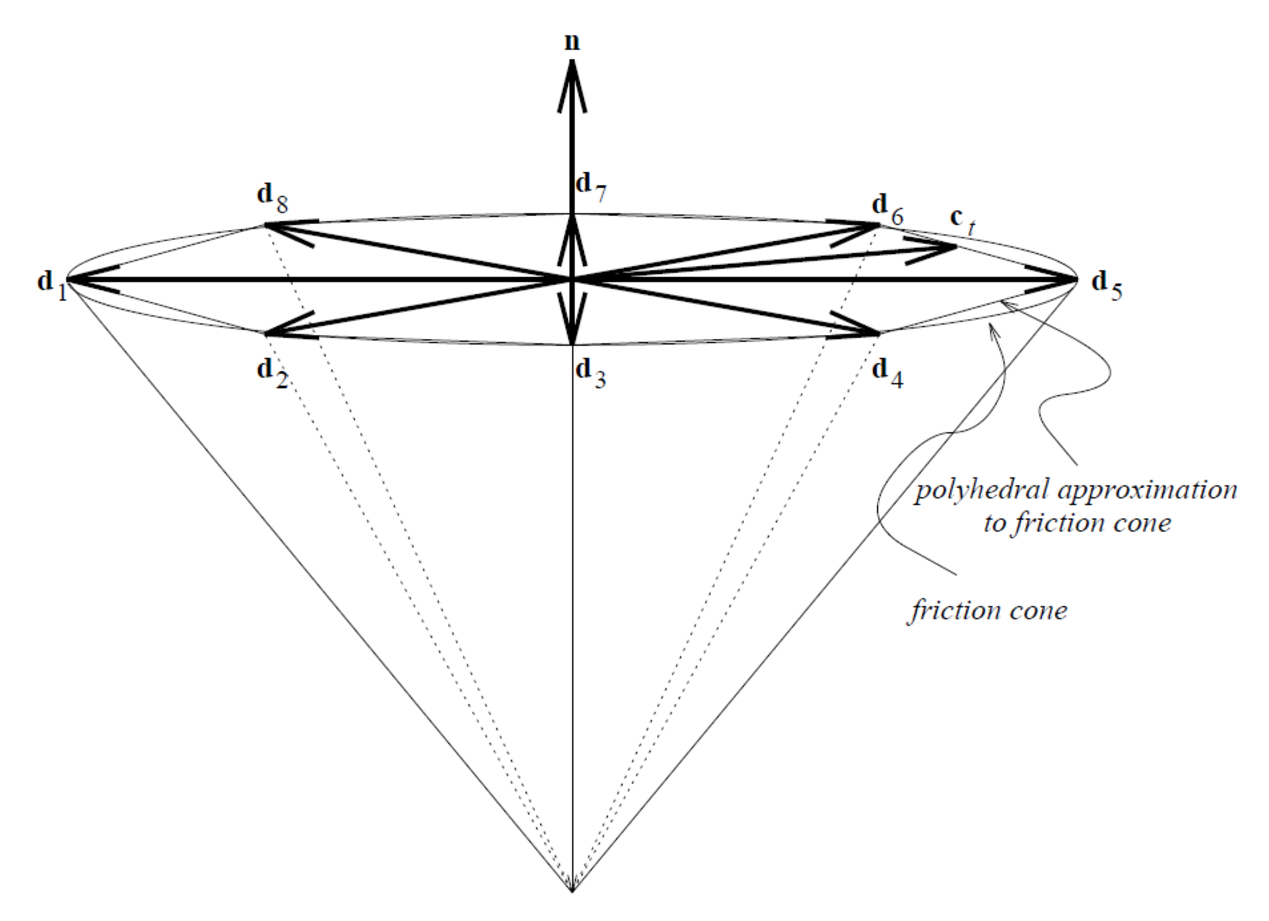
\includegraphics[keepaspectratio=true,height=80mm]{friction_cone.eps}
    \caption{摩擦円錐の近似}%{}内にタイトルを記入してください
    \label{fig:friction_cone}
  \end{center}
\end{figure}


以降,\cite{IJNME1996Stewart} の記号を用いて,クーロン摩擦の条件の近似をまとめる.
一箇所だけで接触が起こり拘束力がはたらく場合を考える.
$\vq$を一般化座標,
$\vn$を接触面に垂直な方向,
$c_n$を法線方向接触力の大きさ,
とする.
摩擦円錐は,次のような角錐で近似できる(Fig.~1).
\begin{align}
 {\cal{F}} = \{ c_n\vn+\vD\vbeta \mid c_n\ge0,~\vbeta\le\0,~\ve^T\vbeta\le\mu c_n \}
\end{align}
$c_n\vn$が垂直抗力,$\vD\vbeta$が摩擦力である.
ここで,$\ve=[1,\cdots,1]^T$である.
$\vbeta$はベクトルの重みである.
$\vD$は$\vq$に依存する行列である.
$\vD$の列ベクトルは,可能な一般化摩擦力の正の部分空間を張る.
全ての$j$について$\vd_j^T\vs\ge0$が成り立つ場合,ベクトル$\vs=\0$が成り立つ.

元々考えたいモデルでは,動摩擦がはたらいている場合,動摩擦力$\vc_t$はすべり速度$\vv$とは反対方向にはたらく.
また,その大きさは$c_t=\mu c_n$であり,摩擦円錐の縁の値に相当する.
そのため,摩擦円錐に含まれる$\vc_t$の内,最も$\vv^T\vc_t$を小さくするようなものが動摩擦である,と考えることができる.
このことをもとにして,近似モデルでは,$\vv^T\vD\vbeta$を最も小さくするような$\vD\vbeta$を動摩擦力として選ぶ.
また,摩擦角錐の縁の値であることも条件であるため,$\ve^T\vbeta=\mu c_n$が成り立つ.
一方で,動摩擦がはたらいていない時には,$\vv=\0$であり,$\ve^T\vbeta\le\mu c_n$である.
さらに,剛体が貫通しないための位置の条件は,$\vn^T\vq\ge\alpha_0$の形で書ける.
剛体が接触していない場合には厳密に不等式$\vn^T\vq>\alpha_0$が成り立ち,このとき垂直抗力の大きさ$c_n=0$である.

これら垂直抗力・摩擦力の条件の近似を,相補形式で表すと,次のように書ける.
\begin{align}
&(\vn^T\vq-\alpha_0)\ge0,
\hspace{5mm}c_n\ge0,
\hspace{5mm}(\vn^T\vq-\alpha_0)c_n=0\notag\\
&(\nu\ve + \vD^T\vv)\ge\0,
\hspace{5mm}\vbeta\ge\0,
\hspace{5mm}(\nu\ve + \vD^T\vv)^T\vbeta=0\label{approx_coulomb_condition}\\
&(\mu c_n - \ve^T\vbeta)\ge0,
\hspace{5mm}\nu\ge0,
\hspace{5mm}(\mu c_n - \ve^T\vbeta)\nu=0\notag
\end{align}
上の相補条件は,速度レベルの拘束式である.


\section{拘束ソルバー }
\paragraph{力/加速度ベース法・撃力/速度ベース法 \cite{MThesis2005Garstenauer} , Sec.~3.6.1}
先述までの方法では,拘束条件$\vc$の2階微分$\ddot{\vc}$を,運動方程式と連立させて解いた.
これは,力と加速度の間の拘束を破らないように計算する方法である.

他の可能性としては,拘束条件$\vc$の1階微分$\dot{\vc}$を連立させて解くことが考えられる.
$\dot{\vc}$は撃力と速度の間の拘束である.
この方法は撃力/速度ベース法と呼ばれ,一方で先述のような方法は力/加速度ベース法と呼ばれる.
時間$\Delta t$のあいだ拘束力$\lambda$が一定にはたらくとみなす近似を置いている.
力/加速度ベース方法では,拘束力が影響を及ぼすのに位置と速度の更新ステップを待たなければならない.
これに対して撃力/速度ベースの方法では,拘束撃力が得られてすぐに速度が変化する.

\paragraph{逐次法・同時法 \cite{MThesis2005Garstenauer} , Sec.~4.5-4.6}
拘束を解く方法は,逐次法と同時法の2つに分けることができるらしい(まだ詳しくは調べていない).
逐次法では,ひとつひとつの拘束を局所的に扱い,力あるいは撃力を計算する.
同時法では,1ステップの間で,全ての拘束が同時に満たされるような力あるいは撃力を見つける.

先述のペナルティ法は,力ベースの逐次法である.

\paragraph{time-stepping 法}
ODEで用いられているtime-stepping法についてまとめる.
これは,撃力ベースの同時法である(\cite{MThesis2005Garstenauer} Sec.~4.6.3).
この方法の特徴は,力ベース法とは異なり,摩擦あり剛体系を扱っているが Lemke のアルゴリズムで計算可能な解が常にあることである(\cite{IJNME1996Stewart} Sec.~5).
(Lemke法は,LCPを解く一般的なアルゴリズムらしいです)

オイラーステップにより加速度を近似すると,
\begin{align*}
 \dot{\vu} \approx \frac{\vu_+-\vu_-}{\Delta t}
\end{align*}
これを運動方程式に代入すると,
\begin{align*}
 \vM(\vu_+-\vu_-) = \vQ^A \Delta t + \vQ^C \Delta t
\end{align*}
先述の垂直抗力と摩擦のモデルを用い,拘束(\ref{approx_coulomb_condition})と両立させると,
\begin{align}
 \vM(\vu_+-\vu_-) &= \vQ^A \Delta t + \vn c_n \Delta t + \vD \vbeta \Delta t\\
&(\vn^T\vq-\alpha_0)\ge0,
\hspace{5mm}c_n\ge0,
\hspace{5mm}(\vn^T\vq-\alpha_0)c_n=0\notag\\
&(\nu\ve + \vD^T\vv)\ge\0,
\hspace{5mm}\vbeta\ge\0,
\hspace{5mm}(\nu\ve + \vD^T\vv)^T\vbeta=0\notag\\
&(\mu c_n - \ve^T\vbeta)\ge0,
\hspace{5mm}\nu\ge0,
\hspace{5mm}(\mu c_n - \ve^T\vbeta)\nu=0\notag
\end{align}


\section{ODE Wikiのメモ\cite{WebODEWiki}}

\paragraph{\cite{WebODEWiki} Manual: Introduction}
\begin{itemize}
 \item Simulation method: The equations of motion are derived from a Lagrange multiplier velocity based model due to Trinkle/Stewart and Anitescu/Potra.
 \item A first order integrator is being used. It's fast, but not accurate enough for quantitative engineering yet. Higher order integrators will come later.
 \item Choice of time stepping methods: either the standard ``big matrix'' method or the newer iterative QuickStep method can be used.
 \item Contact and friction model: This is based on the Dantzig LCP solver described by Baraff, although ODE implements a faster approximation to the Coloumb friction model.
\end{itemize}

\paragraph{\cite{WebODEWiki} Manual: Concepts}
\begin{itemize}
 \item Joint error and the Error Reduction Parameter (ERP)
\end{itemize}
(略)
There is a mechanism to reduce joint error: during each simulation step each joint applies a special force to bring its bodies back into correct alignment. This force is controlled by the error reduction parameter (ERP), which has a value between 0 and 1.
The ERP specifies what proportion of the joint error will be fixed during the next simulation step. If ERP=0 then no correcting force is applied and the bodies will eventually drift apart as the simulation proceeds. If ERP=1 then the simulation will attempt to fix all joint error during the next time step. However, setting ERP=1 is not recommended, as the joint error will not be completely fixed due to various internal approximations. A value of ERP=0.1 to 0.8 is recommended (0.2 is the default).
(略)
\begin{itemize}
 \item Soft constraint and Constraint Force Mixing (CFM)
\end{itemize}
Most constraints are by nature "hard". This means that the constraints represent conditions that are never violated. (略)

Not all constraints are hard. Some "soft" constraints are designed to be violated. (略)

There are two parameters that control the distinction between hard and soft constraints. The first is the error reduction parameter (ERP) that has already been introduced. The second is the constraint force mixing (CFM) value, that is described below.

(略)
Traditionally the constraint equation for every joint has the form
\begin{align*}
\vJ\vv = \vc
\end{align*}
where $\vv$ is a velocity vector for the bodies involved, $\vJ$ is a "Jacobian" matrix with one row for every degree of freedom the joint removes from the system, and $\vc$ is a right hand side vector. At the next time step, a vector $\vlambda$ is calculated (of the same size as $\vc$) such that the forces applied to the bodies to preserve the joint constraint are:
\begin{align*}
\vF_c = \vJ^T \vlambda
\end{align*}
ODE adds a new twist. ODE's constraint equation has the form
\begin{align*}
\vJ \vv = \vc + \mbox{CFM}\vlambda
\end{align*}
where CFM is a square diagonal matrix.
(略)


\subsection{文献から推測するODE計算方法}
正直なところ,オープンソースだから中を見れば分かる訳だが,それはしんどいので,文献から考えられることをまとめる.

次の三種類の拘束がある.
\begin{itemize}
 \item 等式幾何拘束 ...$\vc_1(\vq)=\0$の形,関節は自由度の方向以外は固定される.
 \item 不等式幾何拘束...$\vc_2(\vq)\ge\0$の形,接触点は,接触面の法線方向へはめり込まない.
 \item 不等式速度拘束...$\vc_3(\vv,\vq)\ge\0$の形,接触面方向への速度と摩擦力にはクーロンの法則が成り立つ.
\end{itemize}
先述のように,ERP/CFMは,拘束式の微分を連立させて解く場合に安定化させる方法である.
(等式・不等式)幾何拘束については,微分したものを劇力ベースの運動方程式と組合わせて解くことができるため,次のように書き換えていると考えられる.
\begin{align*}
 \dot{\vc}_1=\0   &\longrightarrow \dot{\vc}_1+\frac{ERP}{\Delta t}\vc - CFM\vlambda_1 =\0\\
 \dot{\vc}_2\ge\0 &\longrightarrow \dot{\vc}_1+\frac{ERP}{\Delta t}\vc - CFM\vlambda_2 \ge\0
\end{align*}
一方で,(不等式)速度拘束を微分すると加速度が出てくるため,撃力ベース法と直接的に組み合わせる事ができない.
そのため,速度拘束ではERPは扱わず,次式みたいなCFMのみを用いているかも?
\begin{align*}
 \vc_3\ge\0 &\longrightarrow \vc_3 - CFM\vlambda_3\ge\0
\end{align*}


\bibliography{ref}



\end{document}
